\section{Arquitectura Tp1}

A continuación, se presenta la arquitectura relacionada con el Tp1 desarrollado por el equipo.

\centerline{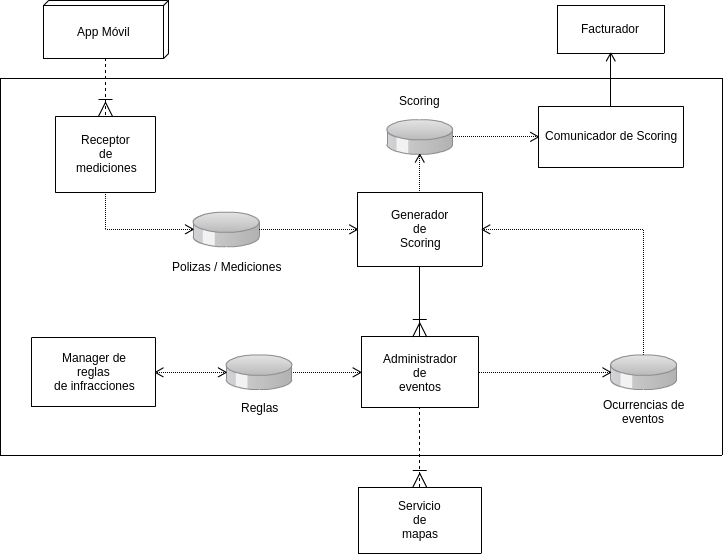
\includegraphics[width=1\textwidth]{./imagenes/tp1.png}}
\centerline{\textit{Figura 10: Arquitectura correspondiente al TP1}}


Como se puede observar, la arquitectura del primer trabajo práctico es bastante más sencilla
que la del segundo. Esto se puede notar debido a la cantidad de componentes que tiene cada una y
las responsabilidades de cada componente.


La arquitectura general del tp1 representa sólo una parte de la del tp2, principalmente la del
\textit{Controlador de Datos de GPS} del \textit{Sistema ManejAR}. 
En particular, el componente \textit{Generador de infracciones} es similar al \textit{Generador de Scoring} en el
sentido que ambos generan infracciones a partir de ciertas reglas preestablecidas.


Por lo tanto, el componente del tp1 está replicado muchas veces en el tp2, ya que en este último caso
hay redundancia en el \textit{Controlador de Datos de GPS} y, dentro de éste, en el \textit{Generador de infracciones}.






